\documentclass[12pt]{article}
\usepackage[utf8]{inputenc}
\usepackage{cite}
\usepackage[utf8]{inputenc}
\usepackage{graphicx}
\usepackage{amsmath}
\usepackage[margin=0.5in]{geometry}
\pagenumbering{gobble}
%\usepackage{geometry}
\usepackage{pdfpages}
\usepackage{xcolor}
\usepackage{todonotes}
\usepackage{amsmath,amsfonts,amssymb,amsthm,epsfig,epstopdf,titling,url,array}
\setcounter{secnumdepth}{4}
%\usepackage{enumerate}% http://ctan.org/pkg/enumerate
\title{Computational Model of Peri-Personal Space}
\author{Joan Reyero}
%\date{\today}


\bibliographystyle{apalike}
%\bibliography{bib}


\begin{document}

\maketitle

\section{Reinforcement learning models}

\subsection{Data exploration}


\begin{figure}[h!]
	\centering
	\hspace*{-0.6in}
	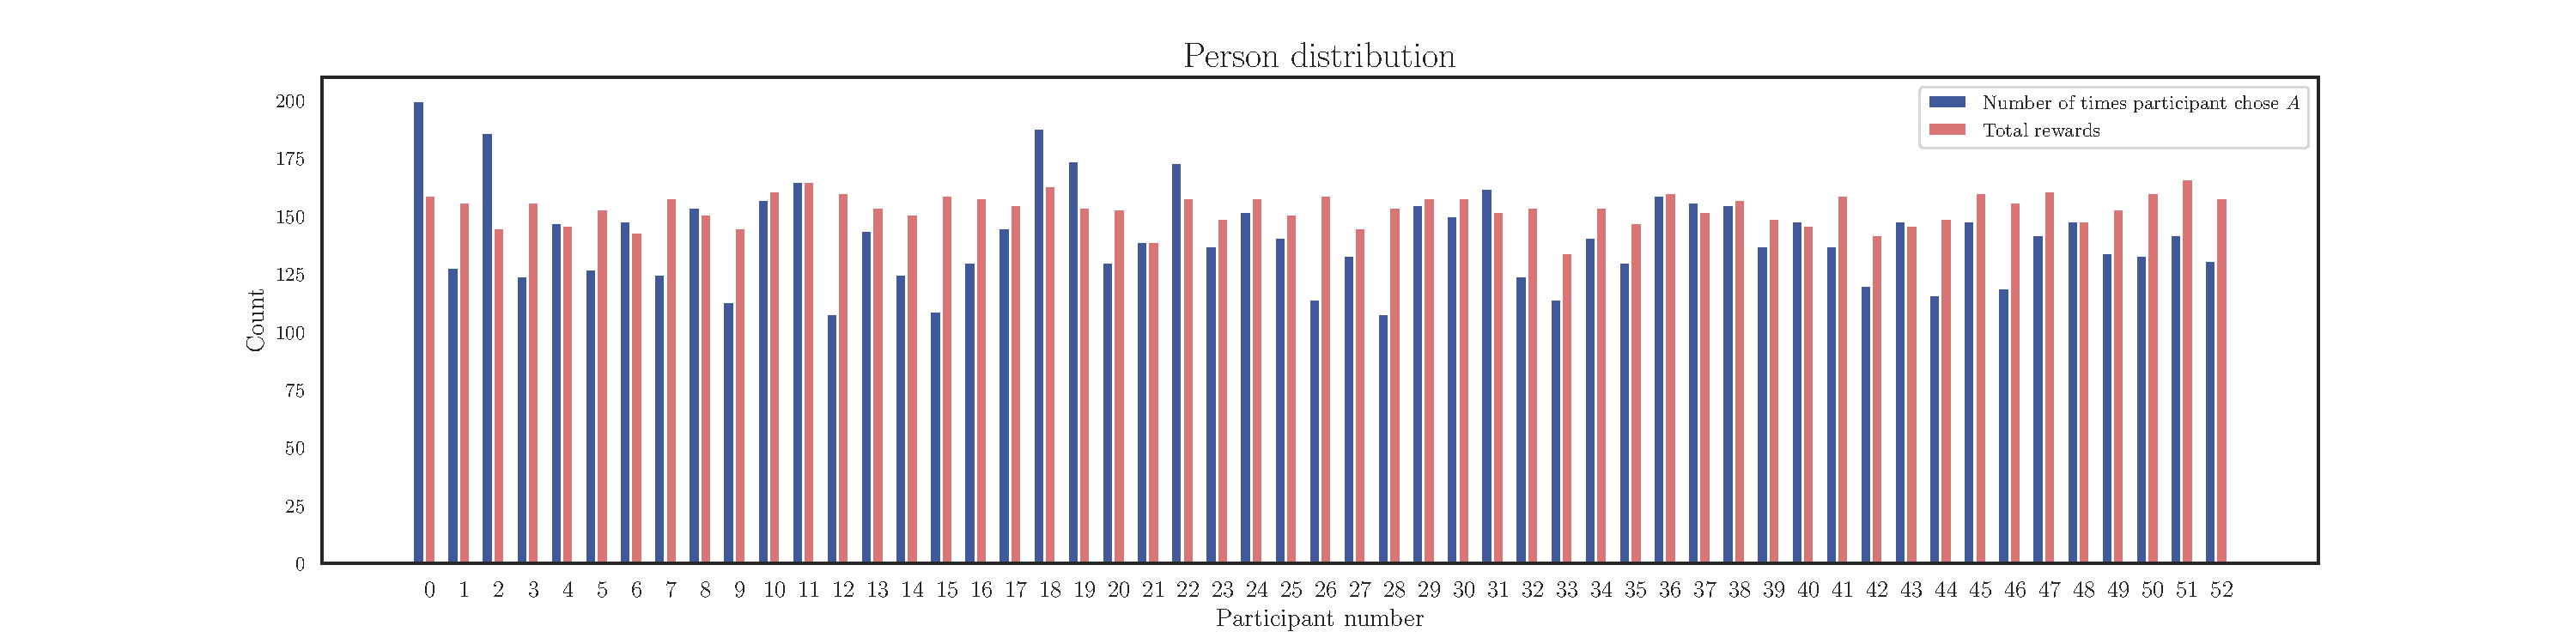
\includegraphics[width=1.2\linewidth]{figures/2.1.pdf}
	\caption{Inputs received by unisensory neurons. (A) Inputs received by auditory-area neurons for a stimulus placed on $(100,5)$cm. (B) Inputs received by tactile-area neurons for a stimulus placed on $(10,5)$cm, the centre of the tactile area.}
	\label{fig:3.1}
\end{figure}

\bibliography{bib}

\end{document}
